\documentclass[border=12pt]{standalone}
\usepackage{tikz}
\usetikzlibrary{shadings,decorations.pathreplacing}

% Colors.
\definecolor{industryC}{HTML}{5EE9B5}
\definecolor{capitalC}{HTML}{F2C14E}
\definecolor{stateC}{HTML}{8EC5FF}

% Parameters.
\def\PyramidH{8}       % apex height
\def\PyramidW{6}       % base half-width
\def\LeaderWidth{2.5}  % width of the leader bar

% Pyramid tiers: base, height of the top end, color.
\def\tiers{%
  Industry/6.2/industryC,%
  The Permanent Overclass/6.5/capitalC,%
  The State/8.0/stateC%
}

\begin{document}
% Half-width of the pyramid at a height `h`: PyramidW * (1 - h/PyramidH)
\newcommand{\hw}[1]{(\PyramidW*(1-(#1)/\PyramidH))}

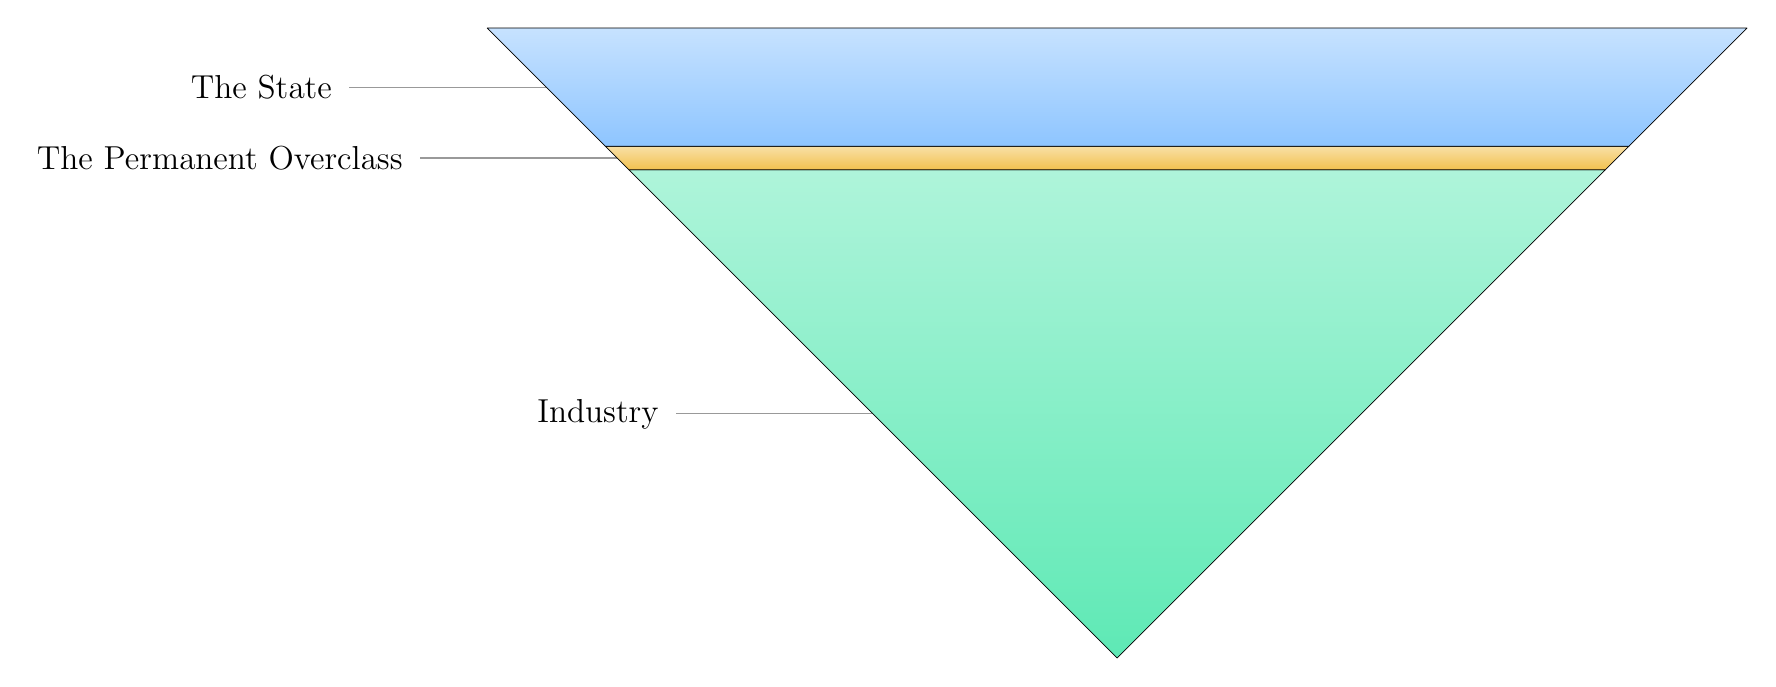
\begin{tikzpicture}[
    line join=round,
    band/.style={draw=black, line width=0.3pt},
    leader/.style={draw=black!40, line width=0.4pt},
    lbl/.style={anchor=east, font=\large},
]

% label geometry, derived from the base width
\pgfmathsetmacro{\LabelX}{-\PyramidW-1}      % right edge of the labels

% Draw each tier.
\foreach \name/\topy/\col [remember=\topy as \prevy (initially 0)] in \tiers {
    % Calculations.
    \pgfmathsetmacro{\mid}{(\prevy+\topy)/2}
    \pgfmathsetmacro{\edge}{-\hw{\mid}}
    % Leader.
    \draw[leader] (\edge, \mid) -- (\edge - \LeaderWidth, \mid);
    % Label.
    \node[lbl] at (\edge - \LeaderWidth - 0.1, \mid) {\name};
    % Trapezoid.
    \shadedraw[band, top color=\col!50, bottom color=\col]
    ({-\hw{\prevy}},\prevy) -- ({\hw{\prevy}},\prevy) --
    ({ \hw{\topy}},\topy)  -- ({-\hw{\topy}},\topy) -- cycle;
}

\end{tikzpicture}
\end{document}
